\begin{center}
\tikzstyle{PoP} = [right,circle, draw]
\tikzstyle{line} = [draw]
\tikzstyle{dotline} = [draw,dotted]
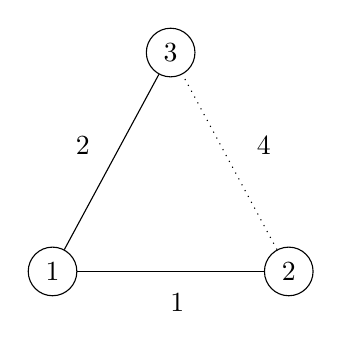
\begin{tikzpicture}
	\node (pop1) at (0.0,0.0) [PoP] {1};
	\node (pop2) at (3.0,0.0) [PoP] {2};
	\node (pop3) at (1.5,2.78) [PoP] {3};
	\path[line](pop1) -- (pop3);
	\path[line](pop1) -- (pop2);
	\path[dotline](pop2) -- (pop3);
	\node  at (0.7,1.6) {2};
	\node  at (1.9,-0.4) {1};
	\node  at (3.0,1.6) {4};
\end{tikzpicture}
\end{center}

